% =====================================================================
%  Northeastern Economics -- Beamer slide template
%  Based on the preamble of M. Shabanpour's conference slides.
%  Compile with pdflatex. Put NULogo.png next to this file to show
%  the logo in the footer (the template compiles without it).
% =====================================================================
\documentclass[aspectratio=169]{beamer}
\usepackage[utf8]{inputenc}
\usepackage{mathpazo}
\usepackage{amsmath,amsfonts,amssymb}
\usepackage{graphicx}
\usepackage[labelformat=empty]{caption}
\usepackage[flushleft]{threeparttable}
\usepackage{booktabs,multirow,makecell,adjustbox,cancel}
\usepackage{tikz}
\usetikzlibrary{positioning,arrows.meta,decorations.pathreplacing}

% Look for figures and tables in the usual project folders
\graphicspath{{./}{Graphs/}{../Graphs/}}
\makeatletter\def\input@path{{./}{Tables/}{../Tables/}}\makeatother

% ---------------- Theme and colours ----------------
\useoutertheme{infolines}
\usetheme{Singapore}
\definecolor{cardinalred}{rgb}{0.2888889, 0.3, 1} % royal blue (name kept from original)
\setbeamercolor{structure}{fg=cardinalred}
\setbeamercovered{transparent}
\setbeamertemplate{navigation symbols}{}
\setbeamertemplate{itemize items}[triangle]
\setlength{\emergencystretch}{2em}

% Section navigation across the top
\setbeamertemplate{headline}{%
  \begin{beamercolorbox}[wd=\dimexpr\paperwidth-2pt\relax,ht=0.6cm,dp=0.4cm,center]{section in head/foot}
    \insertnavigation{\dimexpr\paperwidth-2pt\relax}
  \end{beamercolorbox}}

% Footer: short title | author | logo + slide number
\setbeamertemplate{footline}{%
  \leavevmode\hbox{%
  \begin{beamercolorbox}[wd=.45\paperwidth,ht=2.6ex,dp=1.2ex,left,leftskip=1em]{author in head/foot}\insertshorttitle\end{beamercolorbox}%
  \begin{beamercolorbox}[wd=.35\paperwidth,ht=2.6ex,dp=1.2ex,center]{author in head/foot}\insertshortauthor\end{beamercolorbox}%
  \begin{beamercolorbox}[wd=.20\paperwidth,ht=2.6ex,dp=1.2ex,right,rightskip=.6em]{date in head/foot}%
    \IfFileExists{NULogo.png}{\includegraphics[height=1.8ex]{NULogo.png}\hspace{0.6em}}{}%
    \insertframenumber/\inserttotalframenumber\end{beamercolorbox}}}

% Handy list environments
\newenvironment{wideitemize}{\itemize\addtolength{\itemsep}{10pt}}{\enditemize}
\newenvironment{stepitemize}{\begin{itemize}[<+->]}{\end{itemize}}
\newenvironment{tablefootnotes}{\tiny\begin{flushleft}}{\end{flushleft}}

% ---------------- Title information ----------------
\title[Short Title of Your Paper]{\large Title of Your Paper}
\author[Your Name]{Your Name}
\institute[]{Northeastern University}
\date[]{\today}

\begin{document}

\begin{frame}
  \titlepage
  \vfill
  \begin{center}\scriptsize Prepared for: Conference / Seminar Name\end{center}
\end{frame}

% =====================================================
\section{Introduction}
\begin{frame}{Motivation}
  \begin{wideitemize}
    \item State the economic question in one sentence.
    \item Why it matters: a market, a policy, or a puzzle in the data.
    \item What the existing literature leaves open.
  \end{wideitemize}
\end{frame}

\begin{frame}{This paper}
  \begin{wideitemize}
    \item Contribution 1: data or setting.
    \item Contribution 2: model or identification.
    \pause
    \item Result preview: the headline estimate, with its interpretation.
  \end{wideitemize}
\end{frame}

% =====================================================
\section{Model}
\begin{frame}{Consumer's problem}
\begin{equation}
\begin{aligned}
&\max_{\{x_t,q_t\}_{t=1}^T}\ \sum_{t=1}^T \bigl[u(q_t)+n_t\bigr]\\
&\text{s.t.}\quad \sum_{t=1}^T \bigl(p_t x_t + n_t\bigr)\le T y,\qquad
 l_t=l_{t-1}+x_t-q_t,\quad l_t\ge 0 .
\end{aligned}
\end{equation}
\begin{block}{Intuition}
Explain in one or two lines what the model delivers.
\end{block}
\end{frame}

\begin{frame}{A simple diagram}
\centering
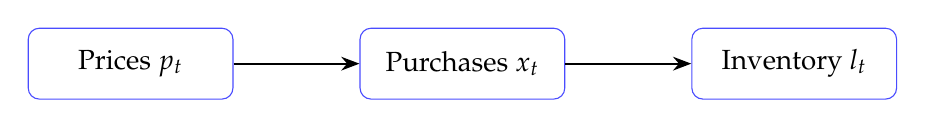
\begin{tikzpicture}[node distance=1.6cm, every node/.style={draw=cardinalred, rounded corners, minimum width=2.6cm, minimum height=0.9cm, align=center}]
  \node (a) {Prices $p_t$};
  \node[right=of a] (b) {Purchases $x_t$};
  \node[right=of b] (c) {Inventory $l_t$};
  \draw[-{Stealth}, thick] (a) -- (b);
  \draw[-{Stealth}, thick] (b) -- (c);
\end{tikzpicture}
\end{frame}

% =====================================================
\section{Results}
\begin{frame}{Main estimates}
\centering
\begin{threeparttable}
\small
\begin{tabular}{lccc}
\toprule
 & (1) & (2) & (3) \\
 & OLS & IV & IV + FE \\
\midrule
Price          & $-0.00$ & $-0.00$ & $-0.00$ \\
               & (0.00)  & (0.00)  & (0.00)  \\
Controls       & No  & Yes & Yes \\
Fixed effects  & No  & No  & Yes \\
\midrule
Observations   & 0 & 0 & 0 \\
\bottomrule
\end{tabular}
\begin{tablefootnotes}
Notes: Placeholder values. Replace with \texttt{\textbackslash input\{table1\}} from your Tables/ folder.
\end{tablefootnotes}
\end{threeparttable}
\end{frame}

% =====================================================
\section{Conclusion}
\begin{frame}{Conclusion}
  \begin{stepitemize}
    \item Main finding.
    \item Mechanism.
    \item Policy or welfare implication.
  \end{stepitemize}
  \vspace{0.3cm}
  \centering\hyperlink{appendix_start}{\beamergotobutton{Appendix}}
\end{frame}

\section{Appendix}
\begin{frame}[label=appendix_start,noframenumbering]{Appendix: estimation details}
  \begin{wideitemize}
    \item Estimator, standard errors, and robustness checks.
  \end{wideitemize}
\end{frame}

\end{document}
